\documentclass[10pt,a4paper]{book}
\usepackage[utf8x]{inputenc}
\usepackage{ucs}
\usepackage{amsmath}
\usepackage{amsfonts}
\usepackage{graphicx}
\makeatletter
\def\ScaleIfNeeded{%
\ifdim\Gin@nat@width>\linewidth
\linewidth
\else
\Gin@nat@width
\fi
}
\makeatother
\usepackage[bookmarksnumbered=true,bookmarksopen=true]{hyperref}
\author{Christian Brandt & Florian Thomas}
\title{Entwicklung webbasierter Software}
\date{Wintersemester 2011/2012}
\begin{document}
\begin{titlepage}
\begin{center}
\begin{figure}[htbp]
\centering

\includegraphics[width=8cm]{Pictures/THM_Logo.png}%
\end{figure}
\large{Fachbereich MNI - Mathematik, Naturwissenschaften \& Informatik}
\linebreak 
\linebreak
\linebreak
\linebreak
\linebreak
\linebreak
\linebreak
\LARGE{Entwicklung webbasierter Software}
\linebreak
\linebreak
\linebreak
\linebreak
\linebreak
\linebreak
\linebreak
\large{Prüfer}
\linebreak
\large{MSc. Martin Karry}
\linebreak
\linebreak
\large{Prüflinge}
\linebreak
\large{Christian Brandt \& Florian Thomas}
\linebreak
\linebreak
\linebreak
\linebreak
\Large{Projekt: Treebook}
\linebreak
\normalsize{Ein soziales Netzwerk mit Anbindung an Facebook und flickr}
\linebreak
\linebreak
\normalsize{Wintersemester 2011/2012}
\begin{figure}[htbp]
\centering

\includegraphics[width=6cm]{Pictures/treebook_treelogo.png}%
\end{figure}
\linebreak
\linebreak
\linebreak
\linebreak
\end{center}
\end{titlepage}
\setcounter{page}{1}
\subsubsection{Eidesstattliche Erklärung}

\tableofcontents
\renewcommand{\chaptername}{}
\renewcommand{\thechapter}{}
\renewcommand{\thesection}{\arabic{section}}
\renewcommand{\thefigure}{\arabic{figure}}

\chapter{Einleitung}
Im Rahmen der Veranstaltung "Entwicklung webbasierter Software", geleitet von Herrn MSc. Martin Karry, soll zum Bestehen eine webbasierte Software entwickelt werden.
\chapter{Einführung}
Die hier beschriebene Software ist ein soziales Netzwerk, vergleichbar mit Facebook\footnote{\href{http://facebook.com/}{http://facebook.com/}} oder Google+\footnote{\href{http://plus.google.com/}{http://plus.google.com/}}. Der Name "Treebook" leitet sich aus der Struktur der Freundschaften innerhalb dieser Software her. Dieses System ist angelehnt an das Circle-System von Google+\footnote{\href{http://www.youtube.com/watch?v=BeMZP-oyOII}{http://www.youtube.com/watch?v=BeMZP-oyOII}}: Der Benutzer (Baum) besitzt mehrere "Trees" (Äste) in denen wiederum mehrere Benutzer enthalten sein können.

Treebook benutzt mehrere Application programming interfaces (nachfolgend kurz API) um die Funktionsmöglichkeiten der Software zu erweitern. Dem Benutzer ist es so mit Hilfe der API von Facebook möglich, sich mit seinen Facebook-Zugangsdaten bei Treebook anzumelden. Die API des Bilderdienstes Flickr\footnote{\href{http://flickr.com}{http://flickr.com}} wird verwendet um dem Anwender zu ermöglichen innerhalb von Treebook mit seinen auf Flickr bereitgestellten Fotos zu interagieren (Fotos ansehen, kommentieren, hochladen).

Der Anwender hat mehrere für ein soziales Netzwerk typische Aktionen zur Auswahl. Er kann Nachrichten (sogenannte "Posts") schreiben, die er mit von ihm ausgewählten "Trees" teilt. Leser einer Nachricht können diese kommentieren, mögen und im Gegensatz zu den bekannten sozialen Netzwerken auch Ablehnung zeigen.

Dem Benutzer steht ein eigenes Profil zur Verfügung in dem er Informationen über sich für die anderen Benutzer veröffentlichen kann. Diese Informationen sowie eventuelle Fotos können über die Privatsphäreneinstellung entweder mit allen angemeldeten Benutzern geteilt werden oder nur mit den eigenen Trees.
\chapter{Analyse}

\chapter{Backend}

\chapter{Frontend}
\section{Allgemeiner Aufbau}
Die Anwendung wird generell in mehreren Schritten geladen. Serverseitig wird zunächst das HTML-Grundgerüst zur Verfügung gestellt, in das nach und nach die gewünschten Inhalte geladen werden.
Dies ermöglichen verschiedene JavaScript-Funktionen, welche neue Informationen per "Asynchronous JavaScript and XML" (kurz AJAX) vom Server abrufen.
Wann und welche Informationen genau vom Server bereitgestellt werden, wird in den folgenden Abschnitten erläutert.

\section{Der Anwendungsstart}
Im Allgemeinen wird beim ersten Besuch der Treebook-Seite die Startseite mit dem Treebook-Logo angezeigt.
\begin{figure}[htbp]
\centering
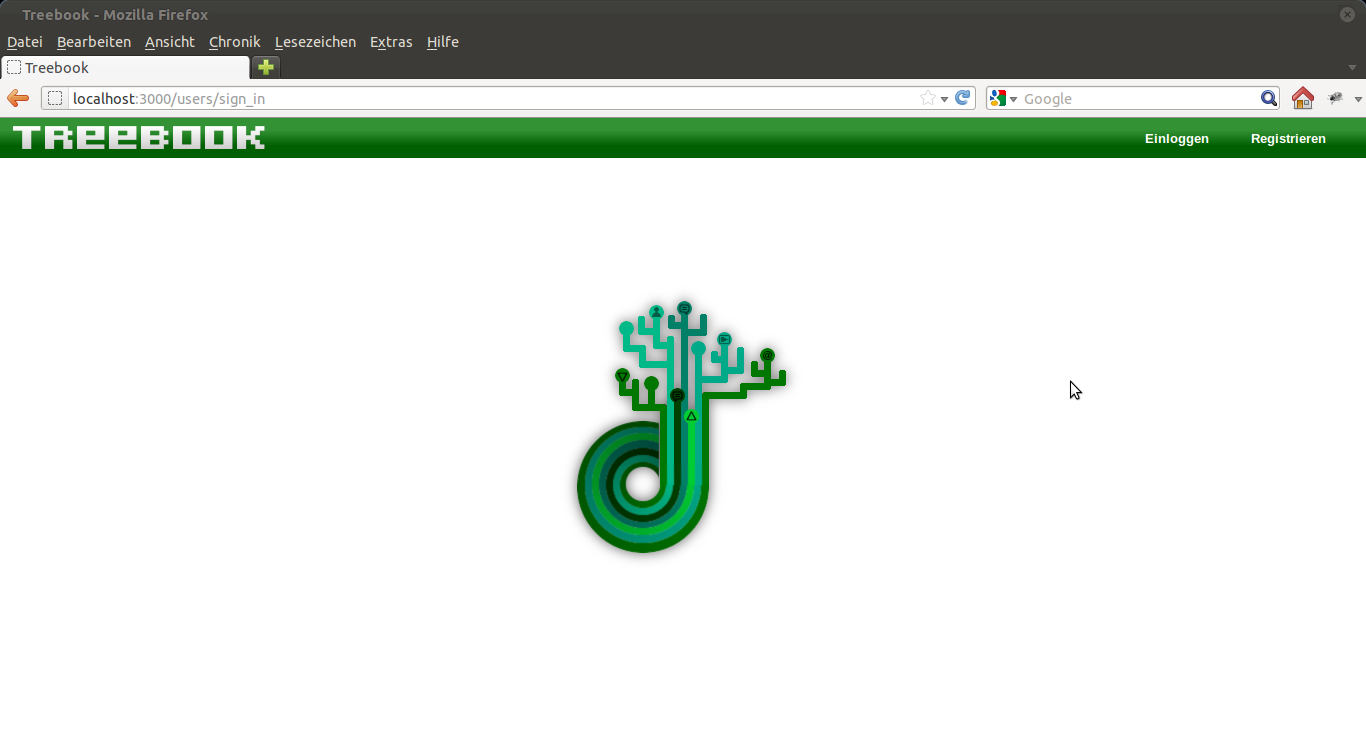
\includegraphics[width=\ScaleIfNeeded]{Pictures/screen_startup.png}%
\caption{Startseite}%
\end{figure}
Von hier aus hat der Anwender die Möglichkeit sich im System anzumelden oder zu registrieren.
Die Anmeldung erfolgt wahlweise über eine dem System bekannte E-Mail-Adresse und dem dazugehörigen Passwort oder über die Facebook-OAuth-API ("Via Facebook anmelden").
Ist der Nutzer dem System noch nicht bekannt, kann er sich dennoch direkt via Facebook anmelden. In diesem Fall wird für ihn ein neues Treebook-Nutzerkonto mit seinen bei Facebook hinterlegten Daten angelegt.

\section{Nach dem Login}
\subsection{Der Stream}
Nachdem sich der Anwender angemeldet hat, sieht er zunächst den sogenannten \textbf{Stream} vor sich. Links davon befindet sich die allgemeine \textbf{Navigation} mit seinen erstellten Trees. Rechts befindet sich ein Suchfeld.
\begin{figure}[htbp]
\centering
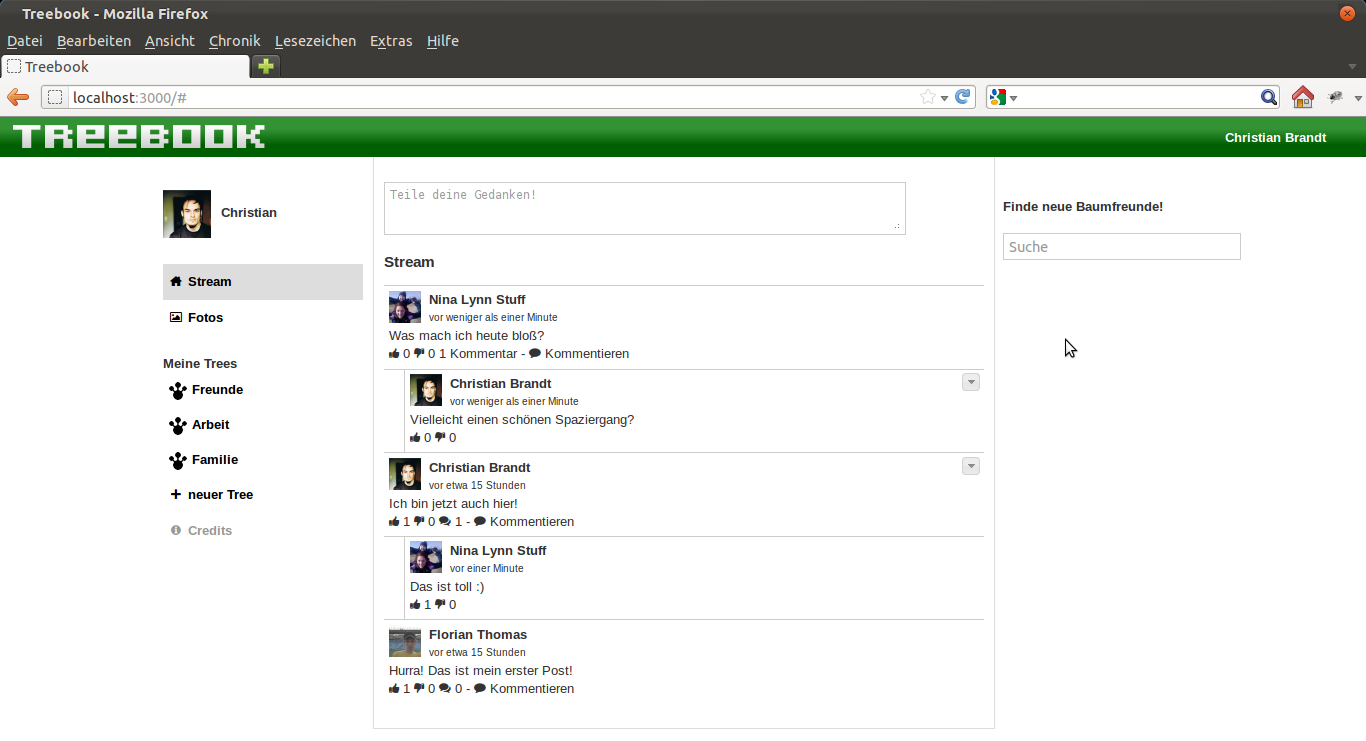
\includegraphics[width=\ScaleIfNeeded]{Pictures/screen_stream.png}%
\caption{Stream}%
\end{figure}
Im Stream werden alle \textbf{Posts} angezeigt, die der Anwender selbst, oder Kontakte in seinen Trees erfasst haben. Diese sind rückwärts sortiert nach Erstellungsdatum, sodass der Anwender am Seitenanfang immer die neuesten Posts sieht und, je weiter er nach unten scrollt, die Posts immer älter werden.
Unter jedem Post werden (sofern vorhanden) die letzten 3 \textbf{Kommentare} zu diesem Post angezeigt. Sind mehr als 3 Kommentare verfügbar, sieht der Anwender einen Link "Alle vorherigen Kommentare anzeigen", welcher nach einem Klick die übrigen Kommentare zum Post anzeigt.
\subsection{Die Navigation}
Die Navigation teilt sich in 4 Unterbereiche auf:
\begin{list}{$\bullet$}{}
\item Das \textbf{Profilbild} und der Vorname des derzeit eingeloggten Nutzers
\item Allgemeine Links zum Stream und zu den \textbf{Fotos} des eingeloggten Nutzers
\item Die vom Nutzer erstellten Trees und ein Link zum Erstellen eines neuen Trees
\item Ein Link zu den \textbf{Credits}
\end{list}
Per Klick auf das Profilbild oder den Vornamen des Anwenders wird das Profil geladen. Standardmäßig sieht der Anwender dann seine eigenen Beiträge aufgelistet.

Mit einem Klick auf "Fotos" wird ebenfalls das Profil des Nutzers geladen, allerdings wird direkt der Foto-Reiter aktiviert.

Klickt der Nutzer auf einen \textbf{Tree}, so werden nur Beiträge angezeigt, die diesem Tree zugeordnet sind, also Beiträge, die vom User explizit für diesen Tree freigegeben wurden, oder Beiträge von Kontakten, die der Nutzer diesem Tree zugeordnet hat.

Ein Klick auf "neuer Tree" zeigt ein Textfeld, in das der Nutzer eine Bezeichnung für den Tree eingibt und zwei Buttons zum Speichern oder Verwerfen des neuen Trees.

Hinter den \textbf{Credits} verbergen sich Links zu Software und sonstigen Ressourcen, die für die Entwicklung von Treebook verwendet wurden.

\subsection{Das Suchfeld}
Das Suchfeld zur Rechten des Streams bietet dem Anwender die Möglichkeit nach Personen zu suchen. Nachdem er mindestens 3 Buchstaben eingetippt hat, liefert das System alle Personen, deren Vor- oder Nachname mit diesen Buchstaben beginnt. Eine Suche nach "Han" wird genauso "Hans Dampf" wie "Lars Hansen" liefern, sofern diese Personen bei Treebook registriert sind.
\begin{figure}[htbp]
\centering
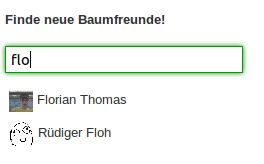
\includegraphics[width=\ScaleIfNeeded]{Pictures/screen_search.png}%
\caption{Suche}%
\end{figure}
Der Anwender hat nun die Möglichkeit per Klick auf einen Namen das Profil des jeweiligen Nutzers aufzurufen, welches dann im mittleren Bereich der Seite angezeigt wird.
Er hat weiterhin die Möglichkeit den Namen per \textbf{Drag and Drop} auf einen Tree in der linken Navigation zu ziehen. Dies fügt den Nutzer dann in den ausgewählten Tree ein, sofern er nicht bereits dem Tree zugeordnet wurde.

\subsection{Der Stream}
Im Stream werden alle Posts und deren Kommentare angezeigt, die vom Nutzer selbst oder seinen Kontakten verfasst wurden. Die Posts sind nach Datum sortiert, wobei die neuesten weiter oben stehen.
Ein Post beinhaltet im Allgemeinen folgende Inhalte:
\begin{list}{$\bullet$}{}
\item Das Profilbild und den vollen Namen des Autors, sowie der ungefähre Zeitraum, der seit dem Veröffentlichen des Posts vergangen ist
\item Den Text, den der Autor verfasst hat
\item Die Anzahl der \textbf{Likes} ("positive Bewertungen"), \textbf{Dislikes} ("negative Bewertungen") und \textbf{Kommentare} zu diesem Post
\item Einen Link zum \textbf{Kommentieren} dieses Posts
\end{list}
\begin{figure}[htbp]
\centering
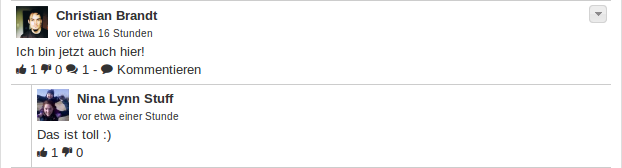
\includegraphics[width=\ScaleIfNeeded]{Pictures/screen_post.png}%
\caption{Post}%
\end{figure}
Sofern der Autor des Posts der aktuelle Nutzer ist, wird in der oberen rechten Ecke des Posts ein kleiner Button mit einem nach unten weisendem Pfeil angezeigt. Bei Klick auf diesen Button öffnet sich ein kleines Kontext-Menü zum \textbf{bearbeiten} und \textbf{löschen} des Posts. Bei erneutem Klick auf den Button wird das Kontext-Menü wieder ausgeblendet.
\begin{figure}[htbp]
\centering
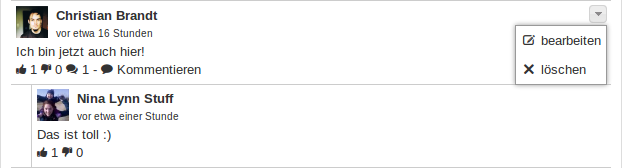
\includegraphics[width=\ScaleIfNeeded]{Pictures/screen_post_menu.png}%
\caption{Post mit Kontext-Menü}%
\end{figure}
Unterhalb des Posts werden die Kommentare eingerückt angezeigt. Diese sind im Wesentlichen genauso aufgebaut, wie ein Post. Allerdings können Kommentare nicht ebenfalls kommentiert werden, daher entfällt die Anzahl der Kommentare und der Link zum Kommentieren.
Standardmäßig werden die bis zu letzten 3 Kommentare zu einem Post angezeigt. Wurde ein Post mehr als dreimal kommentiert, so erscheint zwischen Post und den letzten 3 Kommentaren ein Link "Zeige alle x vorherigen Kommentare", der nachdem er geklickt wurde alle vorherigen Kommentare anzeigt.
\begin{figure}[htbp]
\centering
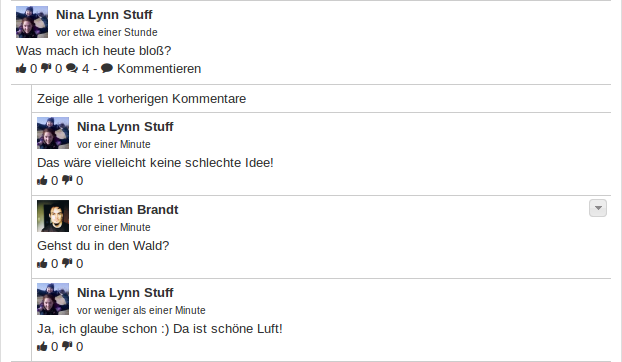
\includegraphics[width=\ScaleIfNeeded]{Pictures/screen_post_and_comments.png}%
\caption{Post mit mehr als 3 Kommentaren}%
\end{figure}
Auch ein Kommentar kann bearbeitet und gelöscht werden, wenn der Nutzer diesen verfasst hat. Dies geschieht analog zur Bearbeitung eines Posts.

\subsection{Die Kopfzeile}
In der Kopfzeile wird zu jeder Zeit der Treebook-Schriftzug angezeigt, der den Link zur Startseite enthält. Am rechten Rand sieht der Nutzer nochmals seinen vollen Namen, hinter dem sich ein Link zu seinem Profil und zum Ausloggen verbirgt.
Nach dem Ausloggen landet der Nutzer wieder auf der Startseite mit dem Treebook-Logo.

\section{Das Profil}
Das Profil eines jeden Nutzers gliedert sich in 3 Bereiche auf:
\begin{list}{$\bullet$}{}
\item Den Kopfbereich, der das Profilbild und den vollen Namen des Nutzers anzeigt
\item Die Profil-Navigation, mit der man zwischen den Beiträgen, den persönlichen Informationen und den Fotos des Nutzers hin- und herschalten kann
\item Die Inhaltsanzeige, die je nach ausgewähltem Pofil-Navigationselement, den entsprechenden nhalt anzeigt
\end{list}

Das Profilbild wird über \textbf{Gravatar}\footnote{\href{http://gravatar.com}{http://gravatar.com}} verwaltet. Betrachtet der Anwender sein eigenes Profil, so erscheint beim Überfahren des Profilsbilds mit der Maus ein kleiner Button zum Bearbeiten des Profilbildes. Dieses verlinkt nach Gravatar, wo der Anwender sein Profilbild ändern kann.

Unter \textbf{Beiträge} sind alle für den Anwender zugänglichen Posts des Nutzers aufgelistet. Posts, die der Anwender nicht sehen soll, wird er auch hier nicht sehen.

Ein Klick auf \textbf{Über mich} zeigt alle persönlichen Profilinformationen des Nutzers, sofern der Anwender sie sehen darf. Besucht der Anwender seine eigene "Über Mich"-Seite, so kann er einerseits seine Privatsphären-Einstellung, andererseits seine persönlichen Profilinformationen bearbeiten.
Die Privatsphären-Einstellung legt fest, welche Treebook-Nutzer seine persönlichen Informationen und seine Fotos sehen dürfen.

Klickt der Anwender auf \textbf{Fotos}, wird er eine der folgenden Inhalte sehen:
\begin{list}{$\bullet$}{}
\item Die Fotos des Nutzers, sofern der Anwender sie sehen darf
\item Einen Hinweis, dass der Nutzer noch keine Fotos erstellt hat
\end{list}
oder, sofern der Anwender ein eigenes Profil aufruft:
\begin{list}{$\bullet$}{}
\item Seine Fotos
\item Einen Hinweis, dass der Anwender jetzt seinen Treebook-Account mit seinem flickr-Konto verknüpfen kann
\end{list}
Wenn Fotos vorhanden sind, werden zunächst nur die Alben des Nutzers als \textbf{Thumbnails} angezeigt. Beim Überfahren mit der Maus erscheinen die bis zu 4 ersten Fotos dieses Albums in einer Miniatur-Ansicht.
Nach Klick auf ein Album werden die enthaltenen Fotos als Thumbnails dargestellt. Zusätzlich wird, wenn das Fotoalbum den Anwender gehört, ein "Plus"-Icon angezeigt, hinter dem sich ein Foto-Upload-Dialog verbirgt.
Nach einem Klick auf ein Foto wird dieses in der Großansicht geöffnet.
In der Großansicht werden außerdem die Kommentare zu diesem Foto sowie ein Formular zum Kommentieren angezeigt. Gehört das Foto dem Anwender, so kann er dessen Titel und Beschreibung bearbeiten.
\chapter{Fazit}

\chapter{Literatur}
\end{document}